%%%%%%%%%%%%%%%%%%%%%%%%%%%%%%%%%%%%%%%%%%%%%%%%%%%%%%%%%%%%%%%%%%%%%%%%%%%%%%%
\section{Introduction}
%%%%%%%%%%%%%%%%%%%%%%%%%%%%%%%%%%%%%%%%%%%%%%%%%%%%%%%%%%%%%%%%%%%%%%%%%%%%%%%
%------------------------------------------------------------------------------
\begin{frame}
  \frametitle{Introduction}
  \begin{itemize}
  \item Widespread usage of multicores and accelerators.
    \begin{itemize}
    \item Highly parallel computing units.
    \item Energy-efficient and low cost devices.
    \end{itemize}

  \item Many applications take advantage of parallel architectures.
  \end{itemize}
  %
  \begin{center}
    \begin{figure}
      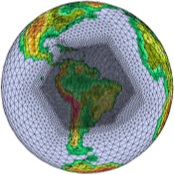
\includegraphics[width=2cm]{olam}
      \hspace{2mm}
      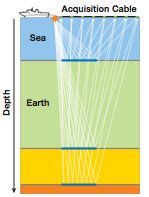
\includegraphics[width=2cm]{seismic}
      \hspace{2mm}
      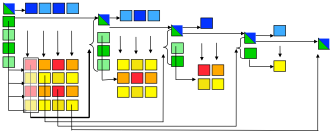
\includegraphics[width=3cm]{fig-lu}
    \end{figure}
  \end{center}
  %
  \begin{itemize}
  \item {\bf Asynchronicity and fine granularity are essential}.
    \begin{itemize}
    \item Avoid/loose synchronizations.
    \item Improve load balancing.
    \item Exploit the available parallelism.
    \end{itemize}
  \end{itemize}
\end{frame}
%------------------------------------------------------------------------------
\begin{frame}
  \frametitle{Introduction}
  \begin{itemize}
  \item {\bf Runtime} - abstraction of the underlying architecture.
    \begin{itemize}
    \item View of parallelism.
    \item View of memory.
    \end{itemize}
  \end{itemize}
  %
  \begin{figure}
  \centering
  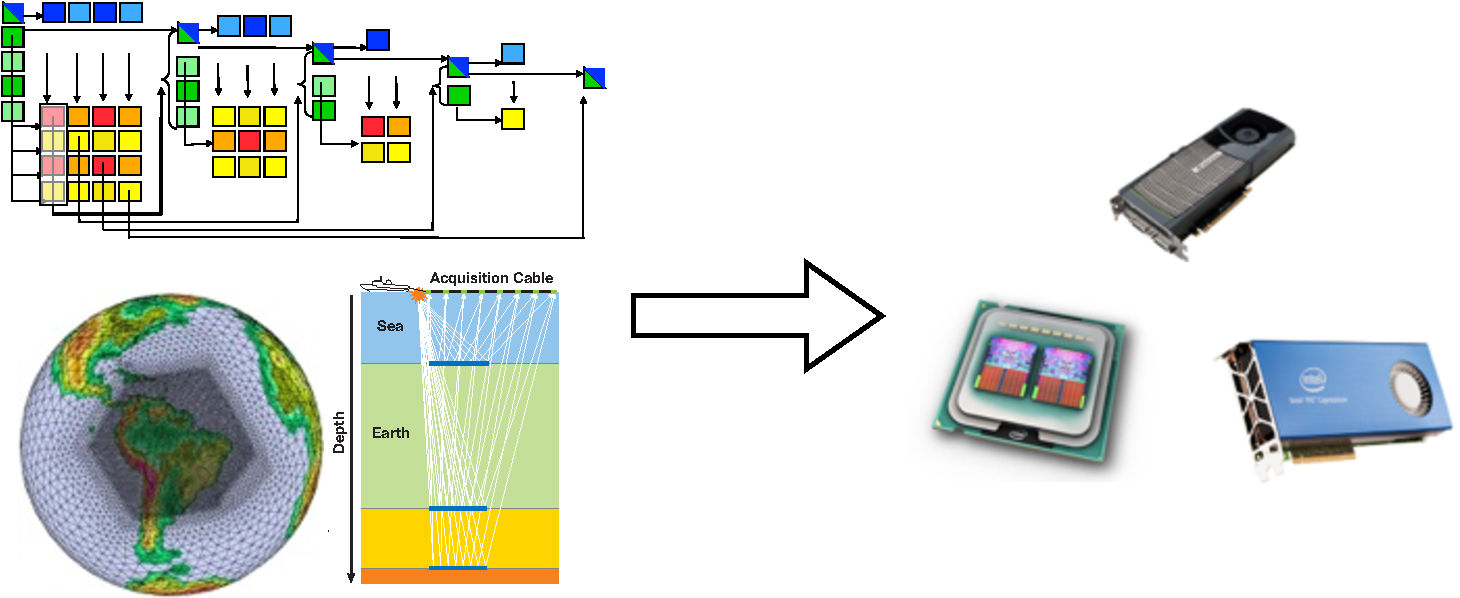
\includegraphics[width=0.8\textwidth]{runtime-system-crop}
  \end{figure}
  %
  \begin{itemize}
  \item {\large In this tutorial we study {\bf data-flow task programming} interfaces.}
  \end{itemize}
\end{frame}
%------------------------------------------------------------------------------
\begin{frame}
  \frametitle{Introduction}
  \begin{exampleblock}{Data-flow task programming}
    Combination of \alert<2->{parallelism} and \alert<2->{memory} view.
    \begin{itemize}
    \item Parallelism is explicit.
    \item Memory view is implicit and \alert<2->{synchronization relies on the runtime}.
    \end{itemize}
  \end{exampleblock}
  %
  \begin{itemize}
  \item Popular in heterogeneous systems.
    \begin{itemize}
    \item A way to express the memory view on disjoint address spaces.
    \end{itemize}
  \item First ``modern'' applications: \blue{tiled algorithms on multicore systems}.
    \begin{itemize}
    \item PLASMA/QUARK from UTK.
    \end{itemize}
  \item Well studied since 1998 with Athapascan/KAAPI (Grenoble/France).
    \begin{itemize}
    \item Now XKaapi.
    \end{itemize}
  \end{itemize}
\end{frame}
%------------------------------------------------------------------------------
